% ------------------------------------------------------------------------------
% TYPO3 CMS 8.3 - What's New (Serbian Version)
%
% @author	Patrick Lobacher <patrick@lobacher.de> and Michael Schams <schams.net>
% @license	Creative Commons BY-NC-SA 3.0
% @link		http://typo3.org/download/release-notes/whats-new/
% @language	Serbian
% ------------------------------------------------------------------------------
% LTXE-CHAPTER-UID:		07b25346-95b1df21-a6ebe09a-49f53f41
% LTXE-CHAPTER-NAME:	Backend User Interface
% ------------------------------------------------------------------------------

\section{Administratorski interfejs}
\begin{frame}[fragile]
	\frametitle{Administratorski interfejs}

	\begin{center}\huge{Poglavlje 1:}\end{center}
	\begin{center}\huge{\color{typo3darkgrey}\textbf{Administratorski interfejs}}\end{center}

\end{frame}

% ------------------------------------------------------------------------------
% LTXE-SLIDE-START
% LTXE-SLIDE-UID:		04db2223-881169a9-2f30301b-8764143a
% LTXE-SLIDE-ORIGIN:	a5b4032f-741b8eea-643674fb-4dc14f50 English
% LTXE-SLIDE-TITLE:		!Feature: #20446 - Clear cache entry in context menu
% LTXE-SLIDE-REFERENCE:	!Feature-20446-ClearCacheEntryInContextMenu.rst
% ------------------------------------------------------------------------------
\begin{frame}[fragile]
	\frametitle{Administratorski interfejs}
	\framesubtitle{"Clear Cache" opcija u kontekst meniju}

	Nova opcija je dodata u kontekst meni od stabla strana. Nalazi se kao podopcija opcije "Page Actions" 
	i dozvoljava da se ocisti kes oznacene strane.

	\begin{figure}
		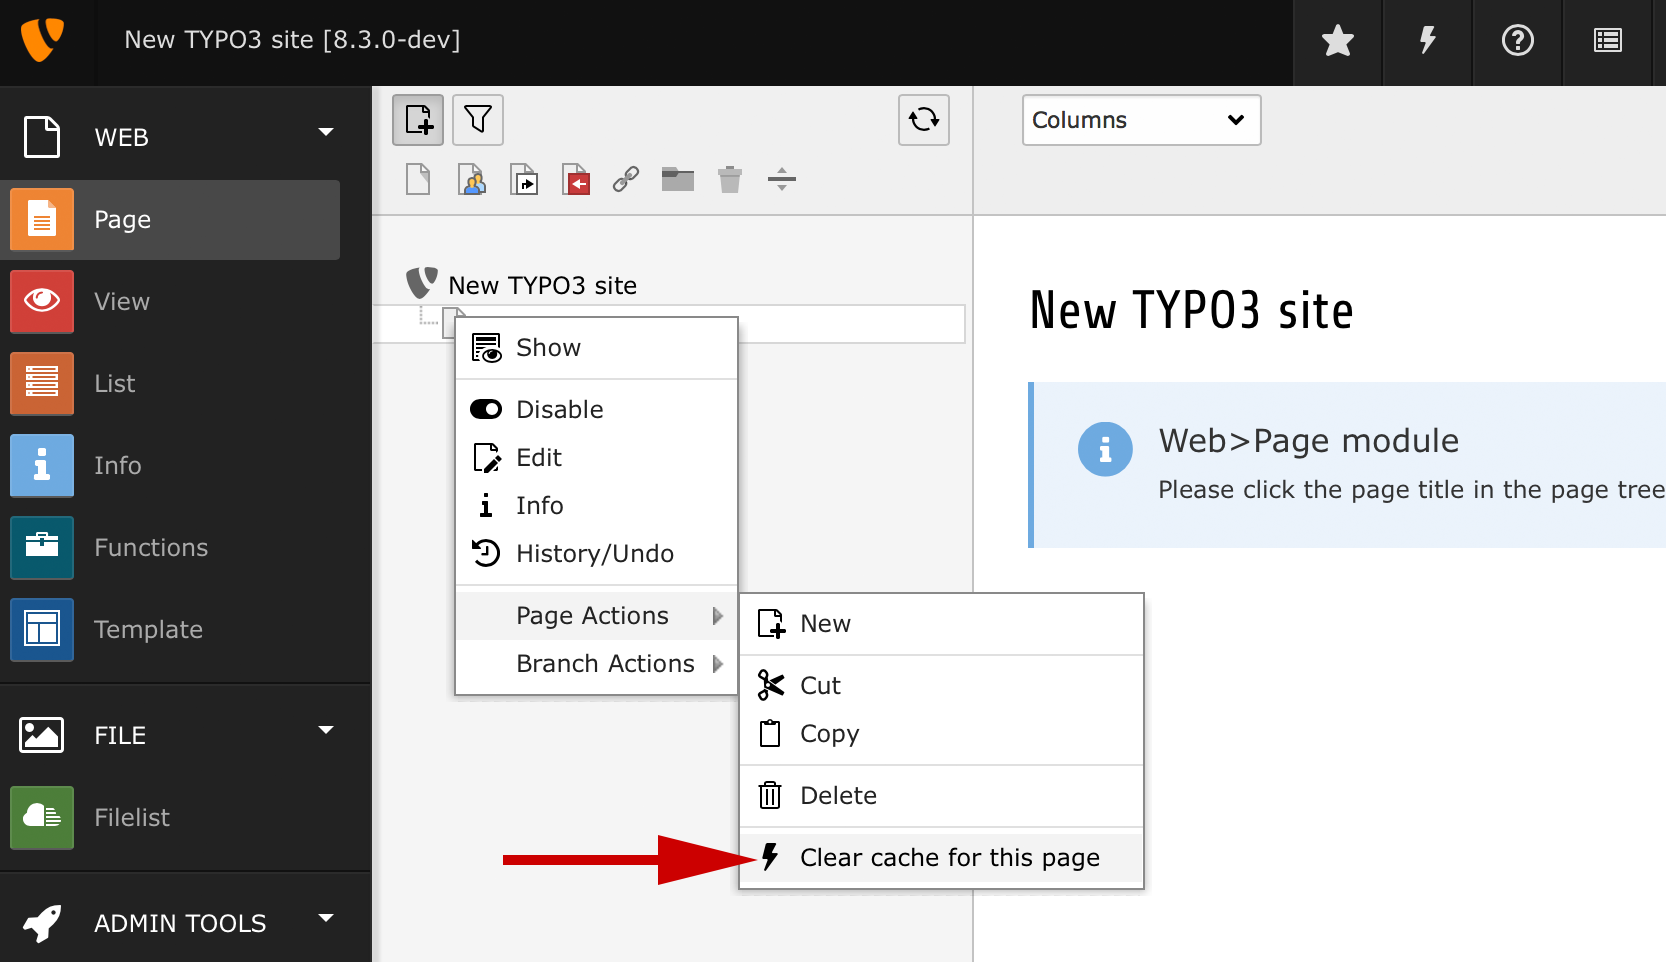
\includegraphics[width=0.70\linewidth]{BackendUserInterface/20446.png}
	\end{figure}

\end{frame}

% ------------------------------------------------------------------------------
% LTXE-SLIDE-START
% LTXE-SLIDE-UID:		4af32435-dd95578d-765cf298-6bf0c96c
% LTXE-SLIDE-ORIGIN:	5b0090eb-13043388-8c4dee34-6cac1521 English
% LTXE-SLIDE-TITLE:		!Feature: #76072 - Ogg, flac and opus support
% LTXE-SLIDE-REFERENCE:	!Feature-76072-OggFlacAndOpusSupport.rst
% ------------------------------------------------------------------------------
\begin{frame}[fragile]
	\frametitle{Administratorski interfejs}
	\framesubtitle{Podrska za Ogg, Flac i Opus}

	U medija polje dodata je podrska za formate:
	\texttt{ogg}, \texttt{flac} i \texttt{opus}

	\begin{figure}
		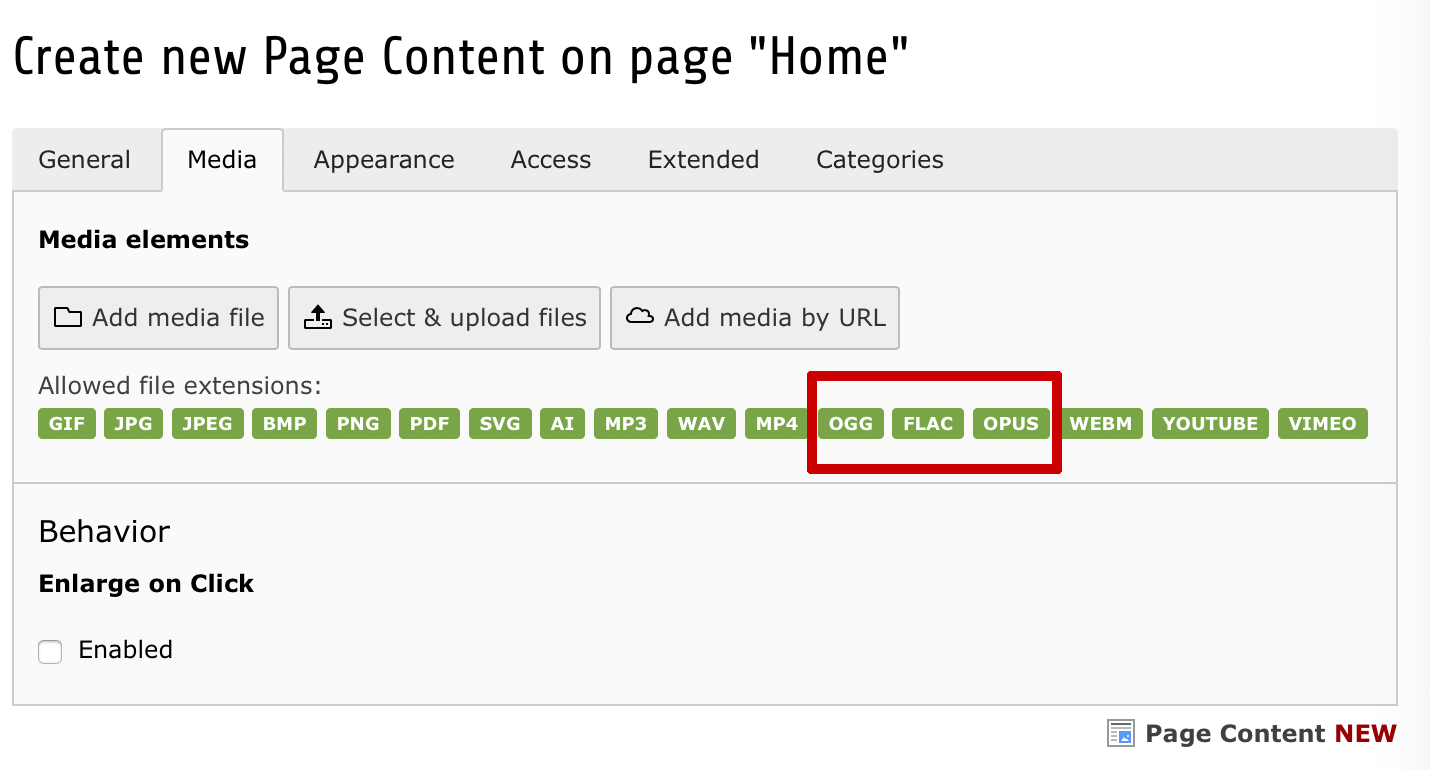
\includegraphics[width=0.70\linewidth]{BackendUserInterface/76072.png}
	\end{figure}

\end{frame}


